\documentclass[11pt]{article}
\renewcommand{\arraystretch}{1.5} % Default value: 1
\usepackage{sectsty}
\allsectionsfont{\color{blue}\fontfamily{lmss}\selectfont}
\usepackage{fontspec}
\setmainfont{XCharter}

\usepackage{listings}
\lstset{
basicstyle=\small\ttfamily,
tabsize=8,
columns=flexible,
breaklines=true,
frame=tb,
rulecolor=\color[rgb]{0.8,0.8,0.7},
backgroundcolor=\color[rgb]{1,1,0.91},
postbreak=\raisebox{0ex}[0ex][0ex]{\ensuremath{\color{red}\hookrightarrow\space}}
}
\usepackage{fontawesome}


\usepackage{mdframed}
\newmdenv[
  backgroundcolor=gray,
  fontcolor=white,
  nobreak=true,
]{terminalinput}



\usepackage{parskip}




    \usepackage[T1]{fontenc}
    % Nicer default font (+ math font) than Computer Modern for most use cases
    \usepackage{mathpazo}

    % Basic figure setup, for now with no caption control since it's done
    % automatically by Pandoc (which extracts ![](path) syntax from Markdown).
    \usepackage{graphicx}
    % We will generate all images so they have a width \maxwidth. This means
    % that they will get their normal width if they fit onto the page, but
    % are scaled down if they would overflow the margins.
    \makeatletter
    \def\maxwidth{\ifdim\Gin@nat@width>\linewidth\linewidth
    \else\Gin@nat@width\fi}
    \makeatother
    \let\Oldincludegraphics\includegraphics
    % Set max figure width to be 80% of text width, for now hardcoded.
\renewcommand{\includegraphics}[1]{\Oldincludegraphics[width=.8\maxwidth, height=.55\textheight, keepaspectratio]{#1}}
    % Ensure that by default, figures have no caption (until we provide a
    % proper Figure object with a Caption API and a way to capture that
    % in the conversion process - todo).
    \usepackage{caption}
    \DeclareCaptionLabelFormat{nolabel}{}
    \captionsetup{labelformat=nolabel, textfont=bf}

    \usepackage{adjustbox} % Used to constrain images to a maximum size
    \usepackage{xcolor} % Allow colors to be defined
    \usepackage{enumerate} % Needed for markdown enumerations to work
    \usepackage{geometry} % Used to adjust the document margins
    \usepackage{amsmath} % Equations
    \usepackage{amssymb} % Equations
    \usepackage{textcomp} % defines textquotesingle
    % Hack from http://tex.stackexchange.com/a/47451/13684:
    \AtBeginDocument{%
        \def\PYZsq{\textquotesingle}% Upright quotes in Pygmentized code
    }
    \usepackage{upquote} % Upright quotes for verbatim code
    \usepackage{eurosym} % defines \euro
    \usepackage[mathletters]{ucs} % Extended unicode (utf-8) support
    \usepackage[utf8x]{inputenc} % Allow utf-8 characters in the tex document
    \usepackage{fancyvrb} % verbatim replacement that allows latex
    \usepackage{grffile} % extends the file name processing of package graphics
                         % to support a larger range
    % The hyperref package gives us a pdf with properly built
    % internal navigation ('pdf bookmarks' for the table of contents,
    % internal cross-reference links, web links for URLs, etc.)
    \usepackage{hyperref}
    \usepackage{longtable} % longtable support required by pandoc >1.10
    \usepackage{booktabs}  % table support for pandoc > 1.12.2
    \usepackage[inline]{enumitem} % IRkernel/repr support (it uses the enumerate* environment)
    \usepackage[normalem]{ulem} % ulem is needed to support strikethroughs (\sout)
                                % normalem makes italics be italics, not underlines




    % Colors for the hyperref package
    \definecolor{urlcolor}{rgb}{0,.145,.698}
    \definecolor{linkcolor}{rgb}{.71,0.21,0.01}
    \definecolor{citecolor}{rgb}{.12,.54,.11}

    % ANSI colors
    \definecolor{ansi-black}{HTML}{3E424D}
    \definecolor{ansi-black-intense}{HTML}{282C36}
    \definecolor{ansi-red}{HTML}{E75C58}
    \definecolor{ansi-red-intense}{HTML}{B22B31}
    \definecolor{ansi-green}{HTML}{00A250}
    \definecolor{ansi-green-intense}{HTML}{007427}
    \definecolor{ansi-yellow}{HTML}{DDB62B}
    \definecolor{ansi-yellow-intense}{HTML}{B27D12}
    \definecolor{ansi-blue}{HTML}{208FFB}
    \definecolor{ansi-blue-intense}{HTML}{0065CA}
    \definecolor{ansi-magenta}{HTML}{D160C4}
    \definecolor{ansi-magenta-intense}{HTML}{A03196}
    \definecolor{ansi-cyan}{HTML}{60C6C8}
    \definecolor{ansi-cyan-intense}{HTML}{258F8F}
    \definecolor{ansi-white}{HTML}{C5C1B4}
    \definecolor{ansi-white-intense}{HTML}{A1A6B2}

    % commands and environments needed by pandoc snippets
    % extracted from the output of `pandoc -s`
    \providecommand{\tightlist}{%
      \setlength{\itemsep}{0pt}\setlength{\parskip}{0pt}}
    \DefineVerbatimEnvironment{Highlighting}{Verbatim}{commandchars=\\\{\}}
    % Add ',fontsize=\small' for more characters per line
    \newenvironment{Shaded}{}{}
    \newcommand{\KeywordTok}[1]{\textcolor[rgb]{0.00,0.44,0.13}{\textbf{{#1}}}}
    \newcommand{\DataTypeTok}[1]{\textcolor[rgb]{0.56,0.13,0.00}{{#1}}}
    \newcommand{\DecValTok}[1]{\textcolor[rgb]{0.25,0.63,0.44}{{#1}}}
    \newcommand{\BaseNTok}[1]{\textcolor[rgb]{0.25,0.63,0.44}{{#1}}}
    \newcommand{\FloatTok}[1]{\textcolor[rgb]{0.25,0.63,0.44}{{#1}}}
    \newcommand{\CharTok}[1]{\textcolor[rgb]{0.25,0.44,0.63}{{#1}}}
    \newcommand{\StringTok}[1]{\textcolor[rgb]{0.25,0.44,0.63}{{#1}}}
    \newcommand{\CommentTok}[1]{\textcolor[rgb]{0.38,0.63,0.69}{\textit{{#1}}}}
    \newcommand{\OtherTok}[1]{\textcolor[rgb]{0.00,0.44,0.13}{{#1}}}
    \newcommand{\AlertTok}[1]{\textcolor[rgb]{1.00,0.00,0.00}{\textbf{{#1}}}}
    \newcommand{\FunctionTok}[1]{\textcolor[rgb]{0.02,0.16,0.49}{{#1}}}
    \newcommand{\RegionMarkerTok}[1]{{#1}}
    \newcommand{\ErrorTok}[1]{\textcolor[rgb]{1.00,0.00,0.00}{\textbf{{#1}}}}
    \newcommand{\NormalTok}[1]{{#1}}

    % Additional commands for more recent versions of Pandoc
    \newcommand{\ConstantTok}[1]{\textcolor[rgb]{0.53,0.00,0.00}{{#1}}}
    \newcommand{\SpecialCharTok}[1]{\textcolor[rgb]{0.25,0.44,0.63}{{#1}}}
    \newcommand{\VerbatimStringTok}[1]{\textcolor[rgb]{0.25,0.44,0.63}{{#1}}}
    \newcommand{\SpecialStringTok}[1]{\textcolor[rgb]{0.73,0.40,0.53}{{#1}}}
    \newcommand{\ImportTok}[1]{{#1}}
    \newcommand{\DocumentationTok}[1]{\textcolor[rgb]{0.73,0.13,0.13}{\textit{{#1}}}}
    \newcommand{\AnnotationTok}[1]{\textcolor[rgb]{0.38,0.63,0.69}{\textbf{\textit{{#1}}}}}
    \newcommand{\CommentVarTok}[1]{\textcolor[rgb]{0.38,0.63,0.69}{\textbf{\textit{{#1}}}}}
    \newcommand{\VariableTok}[1]{\textcolor[rgb]{0.10,0.09,0.49}{{#1}}}
    \newcommand{\ControlFlowTok}[1]{\textcolor[rgb]{0.00,0.44,0.13}{\textbf{{#1}}}}
    \newcommand{\OperatorTok}[1]{\textcolor[rgb]{0.40,0.40,0.40}{{#1}}}
    \newcommand{\BuiltInTok}[1]{{#1}}
    \newcommand{\ExtensionTok}[1]{{#1}}
    \newcommand{\PreprocessorTok}[1]{\textcolor[rgb]{0.74,0.48,0.00}{{#1}}}
    \newcommand{\AttributeTok}[1]{\textcolor[rgb]{0.49,0.56,0.16}{{#1}}}
    \newcommand{\InformationTok}[1]{\textcolor[rgb]{0.38,0.63,0.69}{\textbf{\textit{{#1}}}}}
    \newcommand{\WarningTok}[1]{\textcolor[rgb]{0.38,0.63,0.69}{\textbf{\textit{{#1}}}}}


    % Define a nice break command that doesn't care if a line doesn't already
    % exist.
    \def\br{\hspace*{\fill} \\* }
    % Math Jax compatability definitions
    \def\gt{>}
    \def\lt{<}
    % Document parameters
    \title{answers}




    % Pygments definitions

\makeatletter
\def\PY@reset{\let\PY@it=\relax \let\PY@bf=\relax%
    \let\PY@ul=\relax \let\PY@tc=\relax%
    \let\PY@bc=\relax \let\PY@ff=\relax}
\def\PY@tok#1{\csname PY@tok@#1\endcsname}
\def\PY@toks#1+{\ifx\relax#1\empty\else%
    \PY@tok{#1}\expandafter\PY@toks\fi}
\def\PY@do#1{\PY@bc{\PY@tc{\PY@ul{%
    \PY@it{\PY@bf{\PY@ff{#1}}}}}}}
\def\PY#1#2{\PY@reset\PY@toks#1+\relax+\PY@do{#2}}

\expandafter\def\csname PY@tok@no\endcsname{\def\PY@tc##1{\textcolor[rgb]{0.53,0.00,0.00}{##1}}}
\expandafter\def\csname PY@tok@mh\endcsname{\def\PY@tc##1{\textcolor[rgb]{0.40,0.40,0.40}{##1}}}
\expandafter\def\csname PY@tok@il\endcsname{\def\PY@tc##1{\textcolor[rgb]{0.40,0.40,0.40}{##1}}}
\expandafter\def\csname PY@tok@gd\endcsname{\def\PY@tc##1{\textcolor[rgb]{0.63,0.00,0.00}{##1}}}
\expandafter\def\csname PY@tok@nc\endcsname{\let\PY@bf=\textbf\def\PY@tc##1{\textcolor[rgb]{0.00,0.00,1.00}{##1}}}
\expandafter\def\csname PY@tok@kr\endcsname{\let\PY@bf=\textbf\def\PY@tc##1{\textcolor[rgb]{0.00,0.50,0.00}{##1}}}
\expandafter\def\csname PY@tok@mo\endcsname{\def\PY@tc##1{\textcolor[rgb]{0.40,0.40,0.40}{##1}}}
\expandafter\def\csname PY@tok@m\endcsname{\def\PY@tc##1{\textcolor[rgb]{0.40,0.40,0.40}{##1}}}
\expandafter\def\csname PY@tok@ch\endcsname{\let\PY@it=\textit\def\PY@tc##1{\textcolor[rgb]{0.25,0.50,0.50}{##1}}}
\expandafter\def\csname PY@tok@o\endcsname{\def\PY@tc##1{\textcolor[rgb]{0.40,0.40,0.40}{##1}}}
\expandafter\def\csname PY@tok@go\endcsname{\def\PY@tc##1{\textcolor[rgb]{0.53,0.53,0.53}{##1}}}
\expandafter\def\csname PY@tok@si\endcsname{\let\PY@bf=\textbf\def\PY@tc##1{\textcolor[rgb]{0.73,0.40,0.53}{##1}}}
\expandafter\def\csname PY@tok@nf\endcsname{\def\PY@tc##1{\textcolor[rgb]{0.00,0.00,1.00}{##1}}}
\expandafter\def\csname PY@tok@err\endcsname{\def\PY@bc##1{\setlength{\fboxsep}{0pt}\fcolorbox[rgb]{1.00,0.00,0.00}{1,1,1}{\strut ##1}}}
\expandafter\def\csname PY@tok@s\endcsname{\def\PY@tc##1{\textcolor[rgb]{0.73,0.13,0.13}{##1}}}
\expandafter\def\csname PY@tok@kp\endcsname{\def\PY@tc##1{\textcolor[rgb]{0.00,0.50,0.00}{##1}}}
\expandafter\def\csname PY@tok@sh\endcsname{\def\PY@tc##1{\textcolor[rgb]{0.73,0.13,0.13}{##1}}}
\expandafter\def\csname PY@tok@kn\endcsname{\let\PY@bf=\textbf\def\PY@tc##1{\textcolor[rgb]{0.00,0.50,0.00}{##1}}}
\expandafter\def\csname PY@tok@kc\endcsname{\let\PY@bf=\textbf\def\PY@tc##1{\textcolor[rgb]{0.00,0.50,0.00}{##1}}}
\expandafter\def\csname PY@tok@gs\endcsname{\let\PY@bf=\textbf}
\expandafter\def\csname PY@tok@mf\endcsname{\def\PY@tc##1{\textcolor[rgb]{0.40,0.40,0.40}{##1}}}
\expandafter\def\csname PY@tok@kt\endcsname{\def\PY@tc##1{\textcolor[rgb]{0.69,0.00,0.25}{##1}}}
\expandafter\def\csname PY@tok@nb\endcsname{\def\PY@tc##1{\textcolor[rgb]{0.00,0.50,0.00}{##1}}}
\expandafter\def\csname PY@tok@cs\endcsname{\let\PY@it=\textit\def\PY@tc##1{\textcolor[rgb]{0.25,0.50,0.50}{##1}}}
\expandafter\def\csname PY@tok@cpf\endcsname{\let\PY@it=\textit\def\PY@tc##1{\textcolor[rgb]{0.25,0.50,0.50}{##1}}}
\expandafter\def\csname PY@tok@ne\endcsname{\let\PY@bf=\textbf\def\PY@tc##1{\textcolor[rgb]{0.82,0.25,0.23}{##1}}}
\expandafter\def\csname PY@tok@ss\endcsname{\def\PY@tc##1{\textcolor[rgb]{0.10,0.09,0.49}{##1}}}
\expandafter\def\csname PY@tok@nt\endcsname{\let\PY@bf=\textbf\def\PY@tc##1{\textcolor[rgb]{0.00,0.50,0.00}{##1}}}
\expandafter\def\csname PY@tok@s2\endcsname{\def\PY@tc##1{\textcolor[rgb]{0.73,0.13,0.13}{##1}}}
\expandafter\def\csname PY@tok@sx\endcsname{\def\PY@tc##1{\textcolor[rgb]{0.00,0.50,0.00}{##1}}}
\expandafter\def\csname PY@tok@w\endcsname{\def\PY@tc##1{\textcolor[rgb]{0.73,0.73,0.73}{##1}}}
\expandafter\def\csname PY@tok@sr\endcsname{\def\PY@tc##1{\textcolor[rgb]{0.73,0.40,0.53}{##1}}}
\expandafter\def\csname PY@tok@ni\endcsname{\let\PY@bf=\textbf\def\PY@tc##1{\textcolor[rgb]{0.60,0.60,0.60}{##1}}}
\expandafter\def\csname PY@tok@gu\endcsname{\let\PY@bf=\textbf\def\PY@tc##1{\textcolor[rgb]{0.50,0.00,0.50}{##1}}}
\expandafter\def\csname PY@tok@na\endcsname{\def\PY@tc##1{\textcolor[rgb]{0.49,0.56,0.16}{##1}}}
\expandafter\def\csname PY@tok@cm\endcsname{\let\PY@it=\textit\def\PY@tc##1{\textcolor[rgb]{0.25,0.50,0.50}{##1}}}
\expandafter\def\csname PY@tok@cp\endcsname{\def\PY@tc##1{\textcolor[rgb]{0.74,0.48,0.00}{##1}}}
\expandafter\def\csname PY@tok@c\endcsname{\let\PY@it=\textit\def\PY@tc##1{\textcolor[rgb]{0.25,0.50,0.50}{##1}}}
\expandafter\def\csname PY@tok@mb\endcsname{\def\PY@tc##1{\textcolor[rgb]{0.40,0.40,0.40}{##1}}}
\expandafter\def\csname PY@tok@ow\endcsname{\let\PY@bf=\textbf\def\PY@tc##1{\textcolor[rgb]{0.67,0.13,1.00}{##1}}}
\expandafter\def\csname PY@tok@ge\endcsname{\let\PY@it=\textit}
\expandafter\def\csname PY@tok@kd\endcsname{\let\PY@bf=\textbf\def\PY@tc##1{\textcolor[rgb]{0.00,0.50,0.00}{##1}}}
\expandafter\def\csname PY@tok@gt\endcsname{\def\PY@tc##1{\textcolor[rgb]{0.00,0.27,0.87}{##1}}}
\expandafter\def\csname PY@tok@sb\endcsname{\def\PY@tc##1{\textcolor[rgb]{0.73,0.13,0.13}{##1}}}
\expandafter\def\csname PY@tok@bp\endcsname{\def\PY@tc##1{\textcolor[rgb]{0.00,0.50,0.00}{##1}}}
\expandafter\def\csname PY@tok@nv\endcsname{\def\PY@tc##1{\textcolor[rgb]{0.10,0.09,0.49}{##1}}}
\expandafter\def\csname PY@tok@s1\endcsname{\def\PY@tc##1{\textcolor[rgb]{0.73,0.13,0.13}{##1}}}
\expandafter\def\csname PY@tok@sc\endcsname{\def\PY@tc##1{\textcolor[rgb]{0.73,0.13,0.13}{##1}}}
\expandafter\def\csname PY@tok@nl\endcsname{\def\PY@tc##1{\textcolor[rgb]{0.63,0.63,0.00}{##1}}}
\expandafter\def\csname PY@tok@nn\endcsname{\let\PY@bf=\textbf\def\PY@tc##1{\textcolor[rgb]{0.00,0.00,1.00}{##1}}}
\expandafter\def\csname PY@tok@gi\endcsname{\def\PY@tc##1{\textcolor[rgb]{0.00,0.63,0.00}{##1}}}
\expandafter\def\csname PY@tok@nd\endcsname{\def\PY@tc##1{\textcolor[rgb]{0.67,0.13,1.00}{##1}}}
\expandafter\def\csname PY@tok@vc\endcsname{\def\PY@tc##1{\textcolor[rgb]{0.10,0.09,0.49}{##1}}}
\expandafter\def\csname PY@tok@gr\endcsname{\def\PY@tc##1{\textcolor[rgb]{1.00,0.00,0.00}{##1}}}
\expandafter\def\csname PY@tok@gp\endcsname{\let\PY@bf=\textbf\def\PY@tc##1{\textcolor[rgb]{0.00,0.00,0.50}{##1}}}
\expandafter\def\csname PY@tok@mi\endcsname{\def\PY@tc##1{\textcolor[rgb]{0.40,0.40,0.40}{##1}}}
\expandafter\def\csname PY@tok@sd\endcsname{\let\PY@it=\textit\def\PY@tc##1{\textcolor[rgb]{0.73,0.13,0.13}{##1}}}
\expandafter\def\csname PY@tok@c1\endcsname{\let\PY@it=\textit\def\PY@tc##1{\textcolor[rgb]{0.25,0.50,0.50}{##1}}}
\expandafter\def\csname PY@tok@se\endcsname{\let\PY@bf=\textbf\def\PY@tc##1{\textcolor[rgb]{0.73,0.40,0.13}{##1}}}
\expandafter\def\csname PY@tok@gh\endcsname{\let\PY@bf=\textbf\def\PY@tc##1{\textcolor[rgb]{0.00,0.00,0.50}{##1}}}
\expandafter\def\csname PY@tok@vi\endcsname{\def\PY@tc##1{\textcolor[rgb]{0.10,0.09,0.49}{##1}}}
\expandafter\def\csname PY@tok@k\endcsname{\let\PY@bf=\textbf\def\PY@tc##1{\textcolor[rgb]{0.00,0.50,0.00}{##1}}}
\expandafter\def\csname PY@tok@vg\endcsname{\def\PY@tc##1{\textcolor[rgb]{0.10,0.09,0.49}{##1}}}

\def\PYZbs{\char`\\}
\def\PYZus{\char`\_}
\def\PYZob{\char`\{}
\def\PYZcb{\char`\}}
\def\PYZca{\char`\^}
\def\PYZam{\char`\&}
\def\PYZlt{\char`\<}
\def\PYZgt{\char`\>}
\def\PYZsh{\char`\#}
\def\PYZpc{\char`\%}
\def\PYZdl{\char`\$}
\def\PYZhy{\char`\-}
\def\PYZsq{\char`\'}
\def\PYZdq{\char`\"}
\def\PYZti{\char`\~}
% for compatibility with earlier versions
\def\PYZat{@}
\def\PYZlb{[}
\def\PYZrb{]}
\makeatother


    % Exact colors from NB
    \definecolor{incolor}{rgb}{0.0, 0.0, 0.5}
    \definecolor{outcolor}{rgb}{0.545, 0.0, 0.0}




    % Prevent overflowing lines due to hard-to-break entities
    \sloppy
    % Setup hyperref package
    \hypersetup{
      breaklinks=true,  % so long urls are correctly broken across lines
      colorlinks=true,
      urlcolor=urlcolor,
      linkcolor=linkcolor,
      citecolor=citecolor,
      }
    % Slightly bigger margins than the latex defaults

    \geometry{verbose,tmargin=1in,bmargin=1in,lmargin=1in,rmargin=1in}



\renewcommand{\PY}[2]{{#2}}
\usepackage{fancyhdr}
\pagestyle{fancy}
\rhead{\color{gray}\sf\small\rightmark}
\lhead{\nouppercase{\color{gray}\sf\small\leftmark}}
\cfoot{\color{gray}\sf\thepage}
\renewcommand{\footrulewidth}{1pt}
\begin{document}






    \section{Group Task 1 Answers}\label{group-task-1-answers}

Given an RNA-Seq experiment with a knocked out gene, you were asked to
answer the following questions:

\begin{itemize}
\item
  \textbf{What is the name of the knock out gene?}
\item
  \textbf{What influence does it have?}
\item
  \textbf{How did you determine those?}
\end{itemize}

    \subsection{Dataset}\label{dataset}

You were given the following files in order to conduct the analysis:

\begin{itemize}
\item
  Wild type sample reads in FASTQ format\\
  \texttt{WT{[}replicate{]}\_{[}1\textbar{}2{]}.fastq.gz}
\item
  Knockout sample reads in FASTQ format\\
  \texttt{KO{[}replicate{]}\_{[}1\textbar{}2{]}.fastq.gz}
\item
  \textit{P. berghi} genome in FASTA format\\
  \texttt{PbANKA\_v3.fasta}
\item
  \textit{P. berghi} transcripts in FASTA format\\
  \texttt{Pb.CDS.fasta}
\item
  \textit{P. berghi} annotations in GFF format\\
  \texttt{PbANKA\_v3.gff3.gz}
\item
  \textit{P. berghi} gene descriptions in TSV format\\
  \texttt{Pb.names.txt}
\item
  R script to run sleuth\\
  \texttt{sleuth.R}
\end{itemize}

\newpage

\subsubsection{Important questions}\label{important-questions}

\textbf{Can you summarise the experimental design?}

The experimental design should explain what each sample represents, i.e.
the conditions that were applied and how many replicates there were. In
this experiment, there are two conditions, wild type (WT) and knock out
(KO), each of which has three biological replicates.



    \begin{longtable}[]{@{}ccc@{}}
\hline
Sample name & Condition & Replicate\tabularnewline
\hline
\endhead
WT & wild type & 1\tabularnewline
WT & wild type & 2\tabularnewline
WT & wild type & 3\tabularnewline
KO & knock out & 1\tabularnewline
KO & knock out & 2\tabularnewline
KO & knock out & 3\tabularnewline
\hline
\end{longtable}

    \subsection{Aligning sample reads to the
genome}\label{aligning-sample-reads-to-the-genome}

\textbf{First, we need to move into the directory containing the data.}

\begin{terminalinput}
\begin{Verbatim}[commandchars=\\\{\}]
\llap{\color{black}\LARGE\faKeyboardO\hspace{1em}} \PY{n+nb}{cd} \PYZti{}/course\PYZus{}data/group\PYZus{}projects/RNASeq\PYZus{}1
\end{Verbatim}
\end{terminalinput}


    \textbf{Then, we need to build our HISAT2 index for the genome.}

\begin{terminalinput}
\begin{Verbatim}[commandchars=\\\{\}]
\llap{\color{black}\LARGE\faKeyboardO\hspace{1em}} hisat2\PYZhy{}build PbANKA\PYZus{}v3.fasta PbANKA\PYZus{}v3\PYZus{}hisat2.idx
\end{Verbatim}
\end{terminalinput}

\newpage

    \textbf{Next, we can use a loop to align all of our sample files to the
genome.}

\textit{Be patient, this will take a while!}

\begin{terminalinput}
\begin{Verbatim}[commandchars=\\\{\}]
\llap{\color{black}\LARGE\faKeyboardO\hspace{1em}} \PY{k}{for} fname in *\PYZus{}1.fastq.gz
        \PY{k}{do}
            \PY{c+c1}{\PYZsh{} Get sample name from file name}
            \PY{n+nv}{sample}\PY{o}{=}\PY{l+s+sb}{`}\PY{n+nb}{echo} \PY{l+s+s2}{\PYZdq{}}\PY{n+nv}{\PYZdl{}fname}\PY{l+s+s2}{\PYZdq{}} \PY{p}{|} cut \PYZhy{}d\PY{l+s+s1}{\PYZsq{}\PYZus{}\PYZsq{}} \PYZhy{}f1\PY{l+s+sb}{`}

            \PY{c+c1}{\PYZsh{} Align sample to genome}
            \PY{n+nb}{echo} \PY{l+s+s2}{\PYZdq{}Aligning sample...\PYZdq{}}\PY{l+s+si}{\PYZdl{}\PYZob{}}\PY{n+nv}{sample}\PY{l+s+si}{\PYZcb{}}
            hisat2 \PYZhy{}\PYZhy{}max\PYZhy{}intronlen \PY{l+m}{10000} \PYZhy{}x PbANKA\PYZus{}v3\PYZus{}hisat2.idx \PY{l+s+se}{\PYZbs{}}
            \PYZhy{}1 \PY{l+s+si}{\PYZdl{}\PYZob{}}\PY{n+nv}{sample}\PY{l+s+si}{\PYZcb{}}\PYZus{}1.fastq.gz \PYZhy{}2 \PY{l+s+si}{\PYZdl{}\PYZob{}}\PY{n+nv}{sample}\PY{l+s+si}{\PYZcb{}}\PYZus{}2.fastq.gz \PY{l+s+se}{\PYZbs{}}
            \PYZhy{}S \PY{l+s+si}{\PYZdl{}\PYZob{}}\PY{n+nv}{sample}\PY{l+s+si}{\PYZcb{}}.sam

            \PY{c+c1}{\PYZsh{} Convert SAM to sorted BAM}
            \PY{n+nb}{echo} \PY{l+s+s2}{\PYZdq{}Converting sample SAM to sorted BAM...\PYZdq{}}\PY{l+s+si}{\PYZdl{}\PYZob{}}\PY{n+nv}{sample}\PY{l+s+si}{\PYZcb{}}
            samtools view \PYZhy{}b \PY{l+s+si}{\PYZdl{}\PYZob{}}\PY{n+nv}{sample}\PY{l+s+si}{\PYZcb{}}.sam \PY{p}{|} \PY{l+s+se}{\PYZbs{}}
            samtools sort \PYZhy{}o \PY{l+s+si}{\PYZdl{}\PYZob{}}\PY{n+nv}{sample}\PY{l+s+si}{\PYZcb{}}.sorted.bam

            \PY{c+c1}{\PYZsh{} Index sorted BAM}
            \PY{n+nb}{echo} \PY{l+s+s2}{\PYZdq{}Indexing sample BAM...\PYZdq{}}\PY{l+s+si}{\PYZdl{}\PYZob{}}\PY{n+nv}{sample}\PY{l+s+si}{\PYZcb{}}
            samtools index \PY{l+s+si}{\PYZdl{}\PYZob{}}\PY{n+nv}{sample}\PY{l+s+si}{\PYZcb{}}.sorted.bam
        \PY{k}{done}
\end{Verbatim}
\end{terminalinput}


    \subsubsection{Important questions}\label{important-questions}

\textbf{What is the overall alignment rate of each of the samples?}

It is important to look at the overall alignment rate (for the genome)
as this can give an idea of whether there are any issues with the
experiment (e.g. contamination - like we saw in the practical).

    \begin{longtable}[]{@{}cc@{}}
\hline
Sample name & Alignment rate\tabularnewline
\hline
\endhead
WT1 & 97.63\%\tabularnewline
WT2 & 83.60\%\tabularnewline
WT3 & 97.83\%\tabularnewline
KO1 & 97.14\%\tabularnewline
KO2 & 88.88\%\tabularnewline
KO3 & 97.12\%\tabularnewline
\hline
\end{longtable}

    This looks good, all of the samples have a relatively similar alignment
rate \textgreater{}80\%.


    \subsection{Visualising the genome
alignments}\label{visualising-the-genome-alignments}

Before you can use IGV to visualise the genome, you must first index the
genome using \texttt{samtools\ faidx}.

\textbf{Index the genome with \texttt{samtools}.}

\begin{terminalinput}
\begin{Verbatim}[commandchars=\\\{\}]
\llap{\color{black}\LARGE\faKeyboardO\hspace{1em}} samtools faidx PbANKA\PYZus{}v3.fasta
\end{Verbatim}
\end{terminalinput}


    Once that's finished, you need to load your genome
(\texttt{PbANKA\_v3.fasta}), annotation (\texttt{PbANKA\_v3.gff3.gz})
and sorted alignment files (\texttt{{[}sample{]}.sorted.bam}) into IGV.

\textbf{First, start IGV.}

\begin{terminalinput}
\begin{Verbatim}[commandchars=\\\{\}]
\llap{\color{black}\LARGE\faKeyboardO\hspace{1em}} igv.sh \PY{p}{\PYZam{}}
\end{Verbatim}
\end{terminalinput}


    \textbf{Load the genome file
\texttt{Genomes\ -\textgreater{}\ Load\ Genome\ from\ File}}

\textbf{Load the annotation (gff) file
\texttt{File\ -\textgreater{}\ Load\ from\ File}}

\textbf{Load the sorted sample BAM files
\texttt{File\ -\textgreater{}\ Load\ from\ File}}

\textbf{Make sure to set the alignment tracks to "squished" and to view
reads as "paired".}

\textbf{Type 'PBANKA\_KO' in the search box and click 'Go'.}

This will give you a view like the one below. Here, we have coloured the
WT coverage plots blue and the KO coverage plots red to make it a little
easier to see the difference.

    \begin{figure}[!h]
\centering
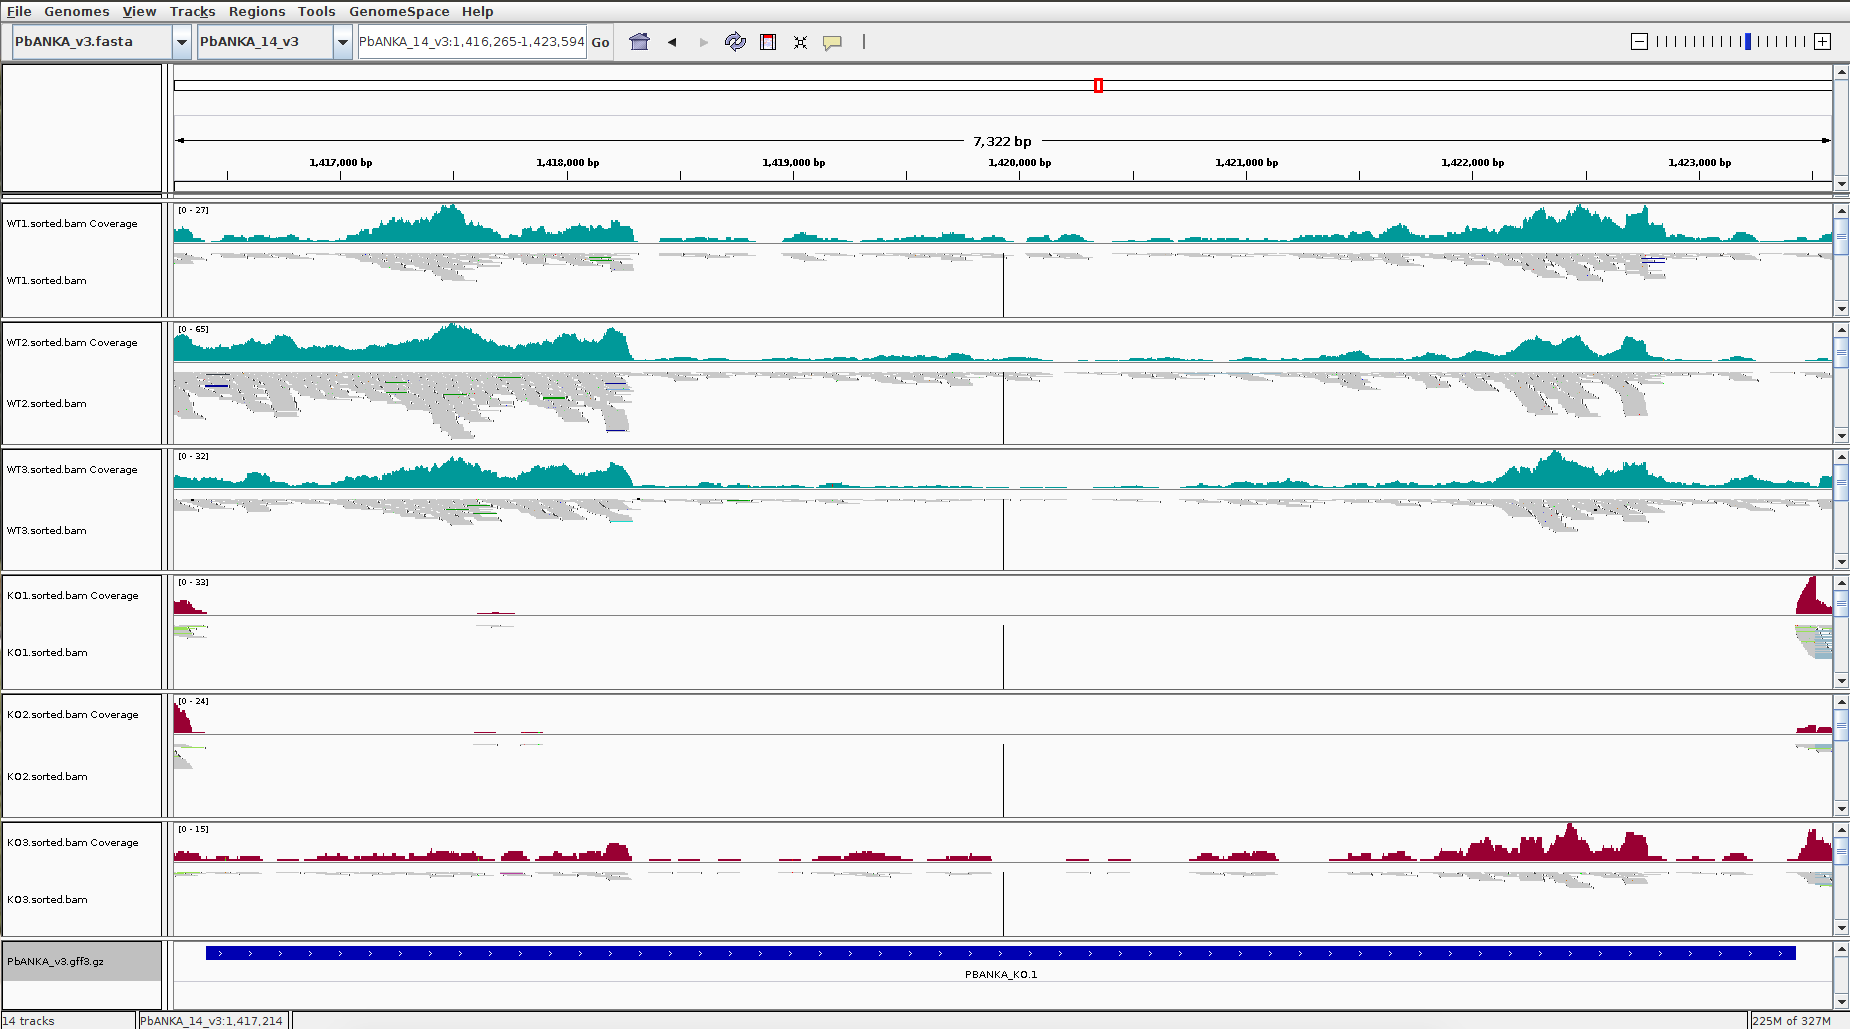
\includegraphics{images/PBANKA_KO_IGV.png}
\caption{images/PBANKA\_KO\_IGV.png}
\end{figure}

    \textbf{Do you notice anything unusual about any of the alignments to
PBANKA\_KO? Should there be any reads mapping to this knocked out gene?}

Here, we've hidden the alignment tracks so that we are just looking at
the coverage plots. As this is a knock out experiment, you would
typically expect to see expression of the gene of interest in the WT
samples and no expression of the gene in the KO samples.

In this case, we can see reads mapping to PBANKA\_KO in our WT samples
as expected. There appears to be a complete knock down in samples KO1
and KO2. However, reads are mapping to PBANKA\_KO in the KO3 sample.
This suggests that it may have been an incomplete knock down of
PBANKA\_KO in KO3.

    \begin{figure}[!h]
\centering
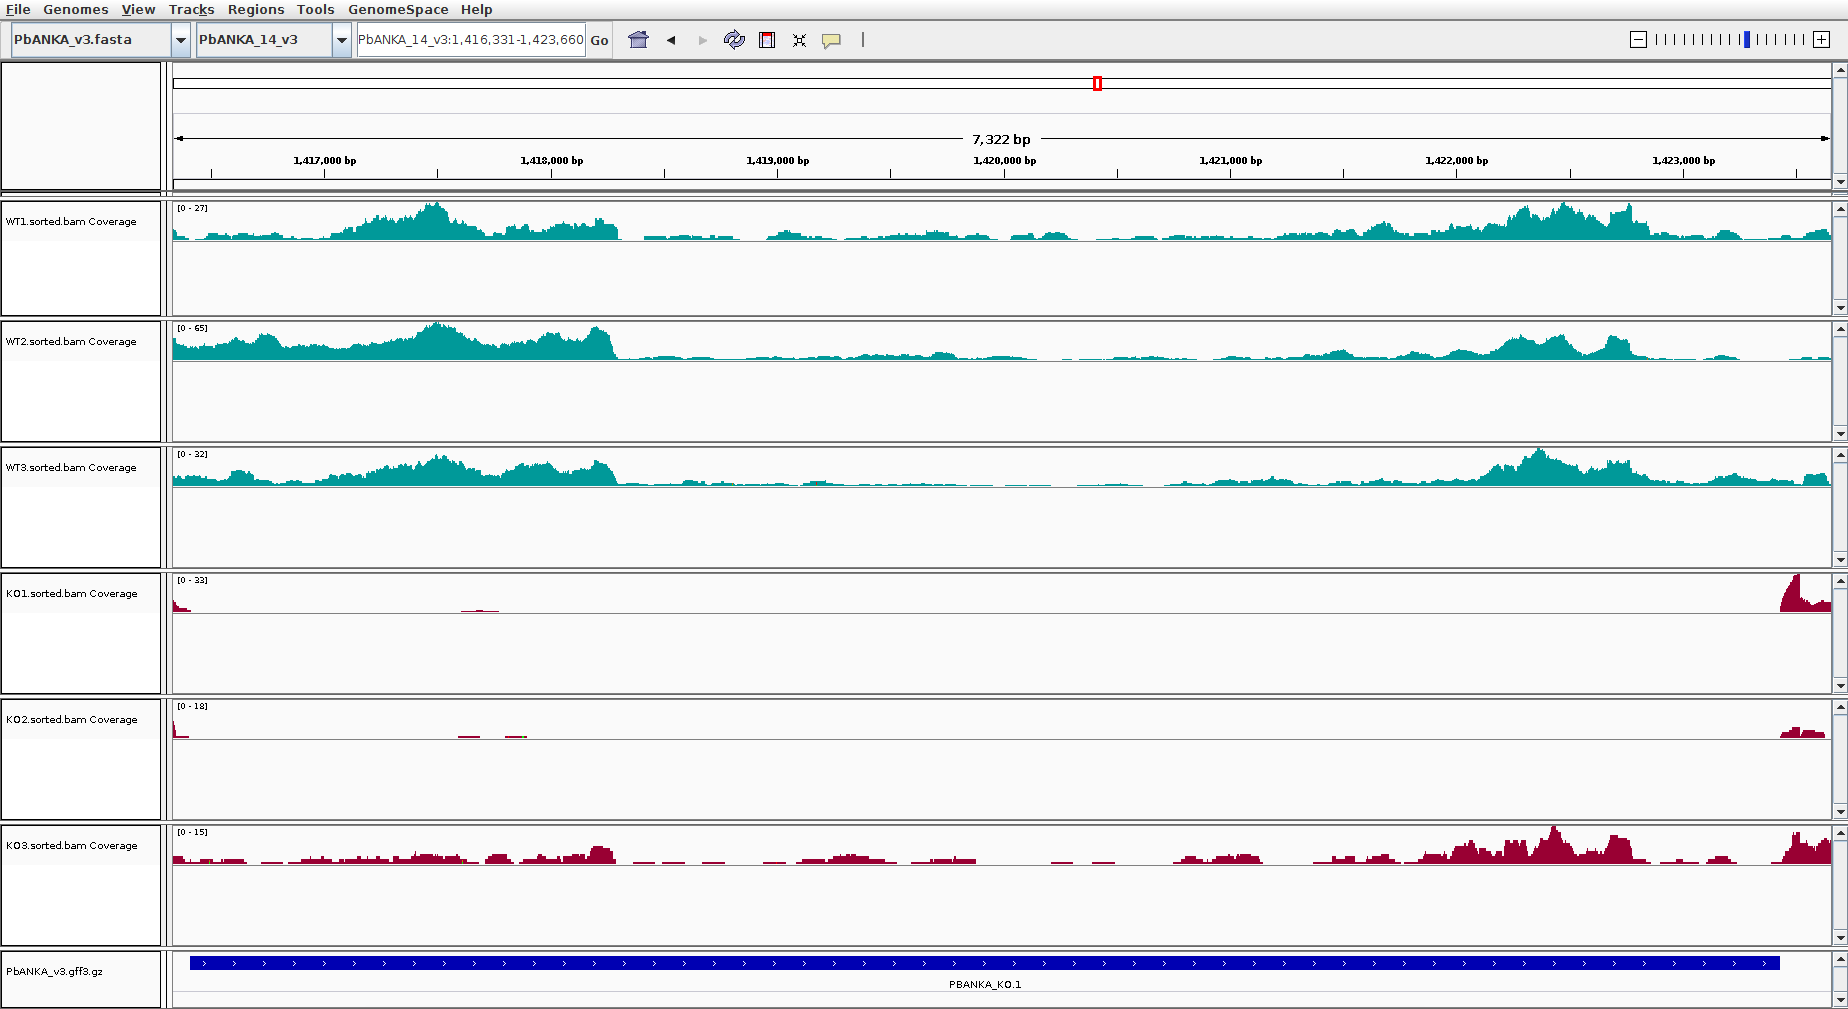
\includegraphics{images/PBANKA_KO_IGV_coverage.png}
\caption{images/PBANKA\_KO\_IGV\_coverage.png}
\end{figure}

    \subsubsection{Important questions}\label{important-questions}

\textbf{Where in the genome is PBANKA\_KO located?}

You can get the co-ordinates of PBANKA\_KO from the annotation file
(\texttt{PbANKA\_v3.gff3.gz}) using \texttt{grep} (first uncompressing
the file with \texttt{gunzip}) or \texttt{zgrep}.

\begin{terminalinput}
\begin{Verbatim}[commandchars=\\\{\}]
\llap{\color{black}\LARGE\faKeyboardO\hspace{1em}} zgrep gene.*PBANKA\PYZus{}KO PbANKA\PYZus{}v3.gff3.gz
\end{Verbatim}
\end{terminalinput}


    PBANKA\_KO is located on the \textbf{forward strand} of
\textbf{PbANKA\_14\_v3} between \textbf{1416412} and \textbf{1423431}.

    \textbf{How many exons does PBANKA\_KO have?}

In IGV, you can see that PBANKA\_KO has \textbf{one exon}.

    \begin{figure}[!h]
\centering

\includegraphics{images/PBANKA_KO_IGV_exon.png}
\caption{images/PBANKA\_KO\_IGV\_exon.png}
\end{figure}

    This can be confirmed by looking for the PBANKA\_KO CDS annotations the
GFF file.

\begin{terminalinput}
\begin{Verbatim}[commandchars=\\\{\}]
\llap{\color{black}\LARGE\faKeyboardO\hspace{1em}} zgrep CDS.*PBANKA\PYZus{}KO PbANKA\PYZus{}v3.gff3.gz
\end{Verbatim}
\end{terminalinput}

    \subsection{Aligning sample reads to the
transcriptome}\label{aligning-sample-reads-to-the-transcriptome}

Before we can use \texttt{kallisto} to align the sample reads to the
transcriptome, we first need to build a kallisto index of the
transcriptome using \texttt{kallisto\ index}.

\textbf{Build a Kallisto index of the tanscriptome
(\texttt{Pb.CDS.fasta}) using \texttt{kallisto}.}

\begin{terminalinput}
\begin{Verbatim}[commandchars=\\\{\}]
\llap{\color{black}\LARGE\faKeyboardO\hspace{1em}} kallisto index \PYZhy{}i Pb.CDS.kallisto Pb.CDS.fasta
\end{Verbatim}
\end{terminalinput}


    As with the genome alignments, we can run the transcriptome alignments
for all the samples using a loop.

\textbf{Align your samples to the transcriptome using
\texttt{kallisto\ quant}.}

\begin{terminalinput}
\begin{Verbatim}[commandchars=\\\{\}]
\llap{\color{black}\LARGE\faKeyboardO\hspace{1em}} \PY{k}{for} fname in *\PYZus{}1.fastq.gz
        \PY{k}{do}
            \PY{c+c1}{\PYZsh{} Get sample name from file name}
            \PY{n+nv}{sample}\PY{o}{=}\PY{l+s+sb}{`}\PY{n+nb}{echo} \PY{l+s+s2}{\PYZdq{}}\PY{n+nv}{\PYZdl{}fname}\PY{l+s+s2}{\PYZdq{}} \PY{p}{|} cut \PYZhy{}d\PY{l+s+s1}{\PYZsq{}\PYZus{}\PYZsq{}} \PYZhy{}f1\PY{l+s+sb}{`}

            \PY{c+c1}{\PYZsh{} Quantify transcript expression in sample}
            \PY{n+nb}{echo} \PY{l+s+s2}{\PYZdq{}kallisto quantification for sample...\PYZdq{}}\PY{l+s+si}{\PYZdl{}\PYZob{}}\PY{n+nv}{sample}\PY{l+s+si}{\PYZcb{}}
            kallisto quant \PYZhy{}i Pb.CDS.kallisto \PYZhy{}o \PY{l+s+si}{\PYZdl{}\PYZob{}}\PY{n+nv}{sample}\PY{l+s+si}{\PYZcb{}} \PYZhy{}b \PY{l+m}{100} \PY{l+s+se}{\PYZbs{}}
            \PY{l+s+si}{\PYZdl{}\PYZob{}}\PY{n+nv}{sample}\PY{l+s+si}{\PYZcb{}}\PYZus{}1.fastq.gz \PY{l+s+si}{\PYZdl{}\PYZob{}}\PY{n+nv}{sample}\PY{l+s+si}{\PYZcb{}}\PYZus{}2.fastq.gz
        \PY{k}{done}
\end{Verbatim}
\end{terminalinput}


    \subsubsection{Important questions}\label{important-questions}

\textbf{How many transcripts are there?}

There are \textbf{5077} transcripts.

\begin{terminalinput}
\begin{Verbatim}[commandchars=\\\{\}]
\llap{\color{black}\LARGE\faKeyboardO\hspace{1em}} grep \PYZhy{}c \PY{l+s+s1}{\PYZsq{}\PYZgt{}\PYZsq{}} Pb.CDS.fasta
\end{Verbatim}
\end{terminalinput}


    \begin{center}\rule{0.5\linewidth}{\linethickness}\end{center}

    \subsection{Run DE analysis in sleuth}\label{run-de-analysis-in-sleuth}

To identify differentially expressed genes you can use the R package,
\texttt{sleuth}.

\textbf{Run the sleuth R script (\texttt{sleuth.R}).}

\begin{terminalinput}
\begin{Verbatim}[commandchars=\\\{\}]
\llap{\color{black}\LARGE\faKeyboardO\hspace{1em}} Rscript sleuth.R
\end{Verbatim}
\end{terminalinput}


    This should give you an error which contains:

\begin{verbatim}
cannot open file 'hiseq_info.txt': No such file or directory
\end{verbatim}

\newpage

\textbf{So, let's take a look at the R script and see what's going on.}

\begin{terminalinput}
\begin{Verbatim}[commandchars=\\\{\}]
\llap{\color{black}\LARGE\faKeyboardO\hspace{1em}} cat sleuth.R
\end{Verbatim}
\end{terminalinput}


    Look at the second line:

\begin{verbatim}
s2c <- read.table("hiseq_info.txt", header = TRUE, stringsAsFactors=FALSE)
\end{verbatim}

The script is looking for a file called \texttt{hiseq\_info.txt}.

\textbf{Let's see if the file has been given to you.}

\begin{terminalinput}
\begin{Verbatim}[commandchars=\\\{\}]
\llap{\color{black}\LARGE\faKeyboardO\hspace{1em}} ls hiseq\PYZus{}info.txt
\end{Verbatim}
\end{terminalinput}


    Nope. Well...we did warn you that some files might be missing! But, that
still doesn't tell us what the \texttt{hiseq\_info.txt} file contains...

\textbf{Let's take a look at the one we used in the practical.}

\begin{terminalinput}
\begin{Verbatim}[commandchars=\\\{\}]
\llap{\color{black}\LARGE\faKeyboardO\hspace{1em}} cat \PYZti{}/pathogen\PYZhy{}informatics\PYZhy{}training/Notebooks/RNA\PYZhy{}Seq/data/hiseq\PYZus{}info.txt
\end{Verbatim}
\end{terminalinput}


    So, it looks like this file indicates which condition was applied to
each of the samples.

\textbf{Copy the file from the practical into the same directory as your
sleuth R script.}

\begin{terminalinput}
\begin{Verbatim}[commandchars=\\\{\}]
\llap{\color{black}\LARGE\faKeyboardO\hspace{1em}} cp \PYZti{}/pathogen\PYZhy{}informatics\PYZhy{}training/Notebooks/RNA\PYZhy{}Seq/data/hiseq\PYZus{}info.txt .
\end{Verbatim}
\end{terminalinput}


    \textbf{Let's check that worked.}

\begin{terminalinput}
\begin{Verbatim}[commandchars=\\\{\}]
\llap{\color{black}\LARGE\faKeyboardO\hspace{1em}} cat hiseq\PYZus{}info.txt
\end{Verbatim}
\end{terminalinput}


    Good, now let's update this file so it contains our sample names.

\textbf{You can edit the file manually by typing the following
\texttt{nano} command in your terminal. Be careful which order you put
the samples in.}

\begin{terminalinput}
\begin{Verbatim}[commandchars=\\\{\}]
\llap{\color{black}\LARGE\faKeyboardO\hspace{1em}} nano \PYZti{}/course\PYZus{}data/group\PYZus{}projects/RNASeq\PYZus{}1/hiseq\PYZus{}info.txt
\end{Verbatim}
\end{terminalinput}


    \textbf{Alternatively, you can make the edits using \texttt{sed}.}

\begin{terminalinput}
\begin{Verbatim}[commandchars=\\\{\}]
\llap{\color{black}\LARGE\faKeyboardO\hspace{1em}} sed \PYZhy{}i \PYZhy{}e \PY{l+s+s1}{\PYZsq{}s/MT/WT/g\PYZsq{}} hiseq\PYZus{}info.txt
        sed \PYZhy{}i \PYZhy{}e \PY{l+s+s1}{\PYZsq{}s/SBP/KO/g\PYZsq{}} hiseq\PYZus{}info.txt
        sed \PYZhy{}ie \PY{l+s+s1}{\PYZsq{}/\PYZca{}WT2/a WT3\PYZbs{}tWT\PYZsq{}} hiseq\PYZus{}info.txt
\end{Verbatim}
\end{terminalinput}


    \textbf{And, check that it's worked.}

\begin{terminalinput}
\begin{Verbatim}[commandchars=\\\{\}]
\llap{\color{black}\LARGE\faKeyboardO\hspace{1em}} cat hiseq\PYZus{}info.txt
\end{Verbatim}
\end{terminalinput}


    Perfect, our six samples are now in the file.

\newpage

\textbf{So, let's try running that R script again.}

\begin{terminalinput}
\begin{Verbatim}[commandchars=\\\{\}]
\llap{\color{black}\LARGE\faKeyboardO\hspace{1em}} Rscript sleuth.R
\end{Verbatim}
\end{terminalinput}


    \textbf{Click \url{http://127.0.0.1:42427} to open the sleuth results in
your web browser.}

    \subsubsection{Important questions}\label{important-questions}

\textbf{Can you summarise the data that's been processed (i.e. number of
reads processed and the proportion of reads mapping to the genome and
transcriptome)?}

You can get a summary of the processed data by going to
\texttt{summaries\ -\textgreater{}\ processed\ data}.

    \begin{figure}[!h]
\centering
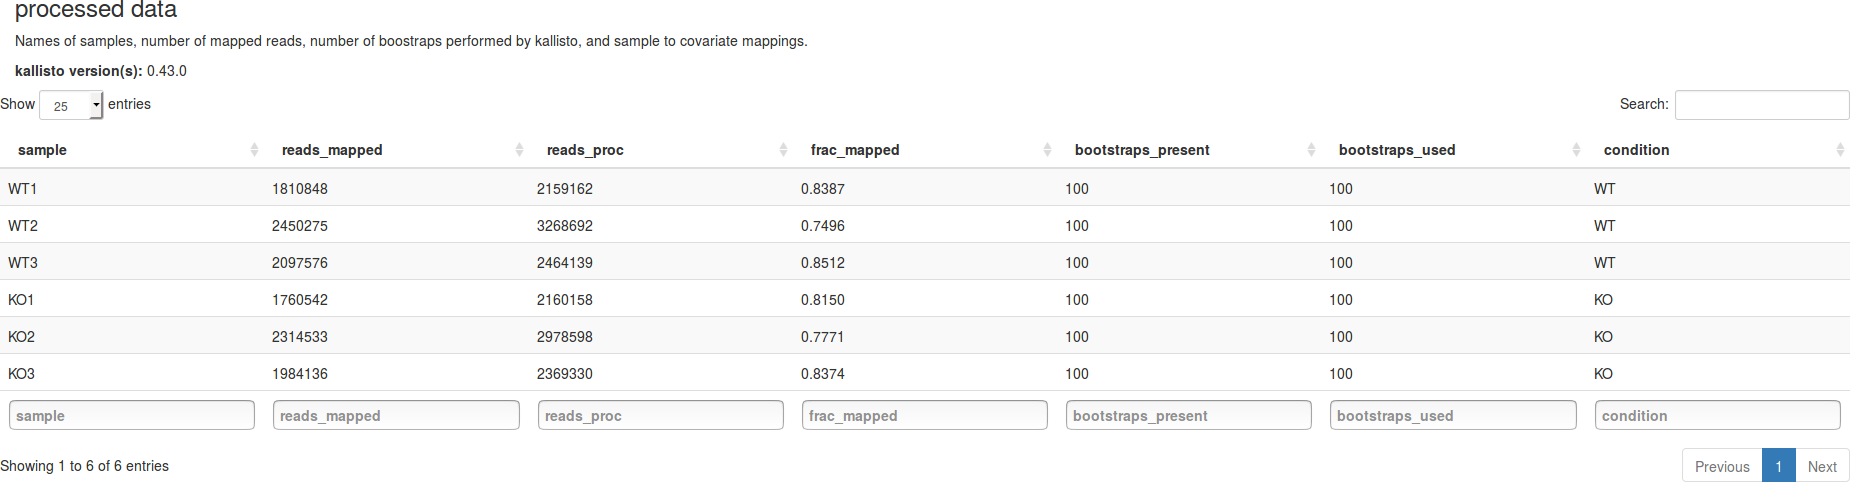
\includegraphics{images/kallisto_processed_data.png}
\caption{images/kallisto\_processed\_data.png}
\end{figure}

    \textbf{Looking at the PCA plot (\texttt{maps\ -\textgreater{}\ PCA}) do
you think the samples form tight, distinct clusters based on the
condition (WT or KO) that was applied?}

Not really. There is a vertical split between the WT and the KO samples.
However, KO3 is reasonably close to the WT samples because of the
incomplete knock out, which prevents tighter clustering.

    \begin{figure}[!h]
\centering
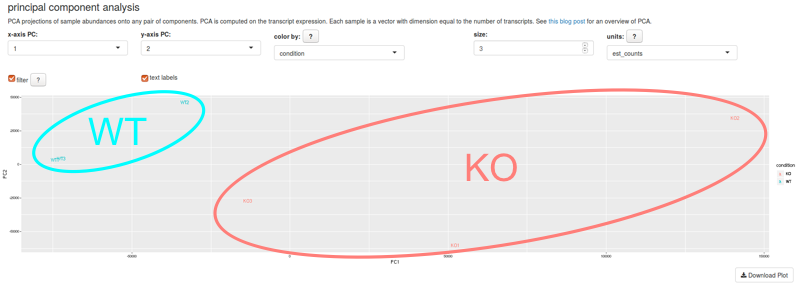
\includegraphics{images/sleuth_original_pca.png}
\caption{images/sleuth\_original\_pca.png}
\end{figure}

    You can also look at the proportion of variance explained by each
principal component (PC). As this is a single factor experiment, we
would expect that if there were variation, most of this would be
explained by the first principal component, PC1. Broadly speaking, this
represents the variation resulting from the difference in condition (WT
vs KO).

\newpage

You can see here that \textgreater{}75\% of the variance is explained by
PC1 (the vertical axis of the PCA plot above). However, there's 15-20\%
of the variance which is explained by the second principal component.
It's possible this is linked to the replicate number and, if you were
particularly worried about it, can be accounted for in downstream
analyses.

    \begin{figure}[!h]
\centering
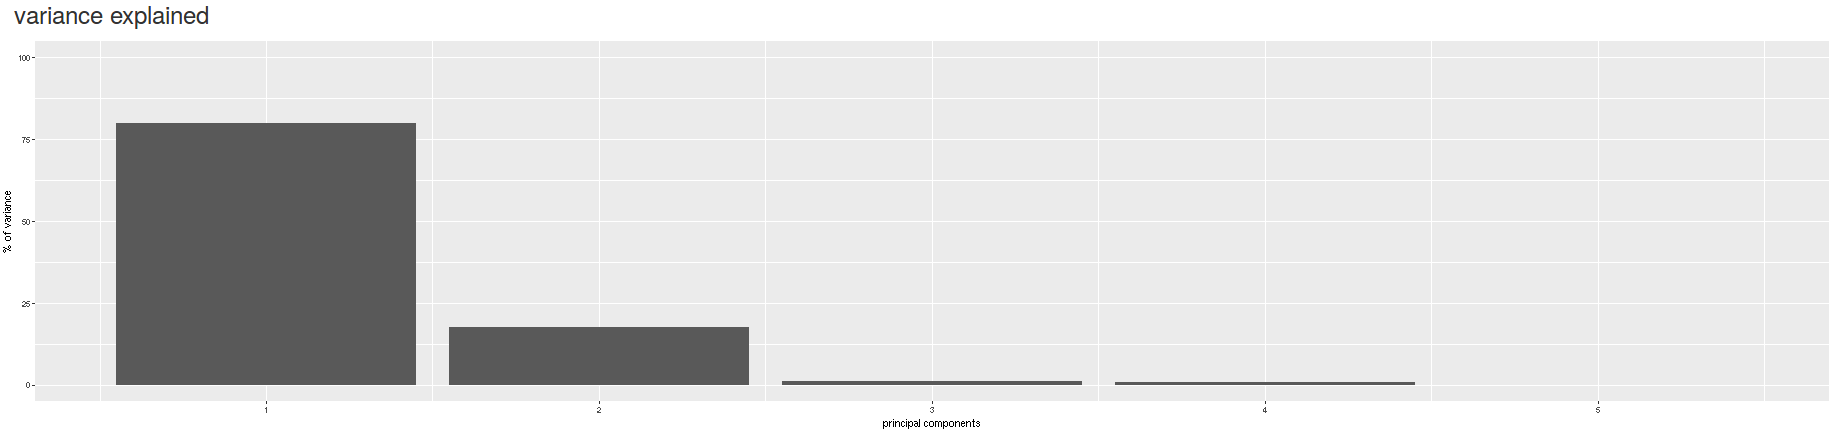
\includegraphics{images/sleuth_original_pca_bar.png}
\caption{images/sleuth\_original\_pca\_bar.png}
\end{figure}

    If you were to rerun the analysis with KO3 removed, the PCA plot does
become a little clearer.

    \begin{figure}[!h]
\centering
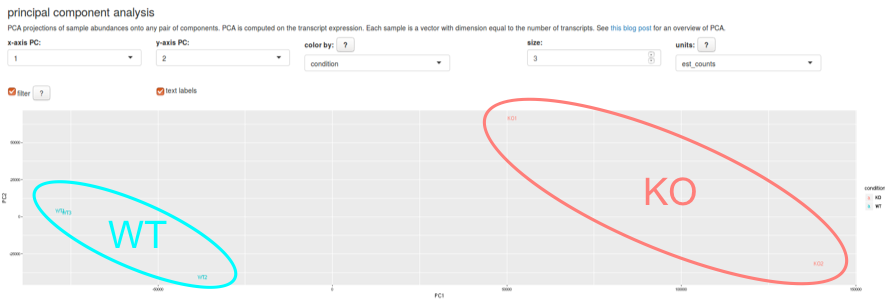
\includegraphics{images/sleuth_processed_pca.png}
\caption{images/sleuth\_processed\_pca.png}
\end{figure}

    \textbf{Was PBANKA\_KO differentially expressed?}

\textbf{Yes} as it's significantly (q-value \textless{} 0.05) more
highly expressed (b \textgreater{} 0) in the WT samples.

For this, you need to go to
\texttt{analyses\ -\textgreater{}\ test\ table} and enter PBANKA\_KO in
the search box.

    \begin{figure}[!h]
\centering
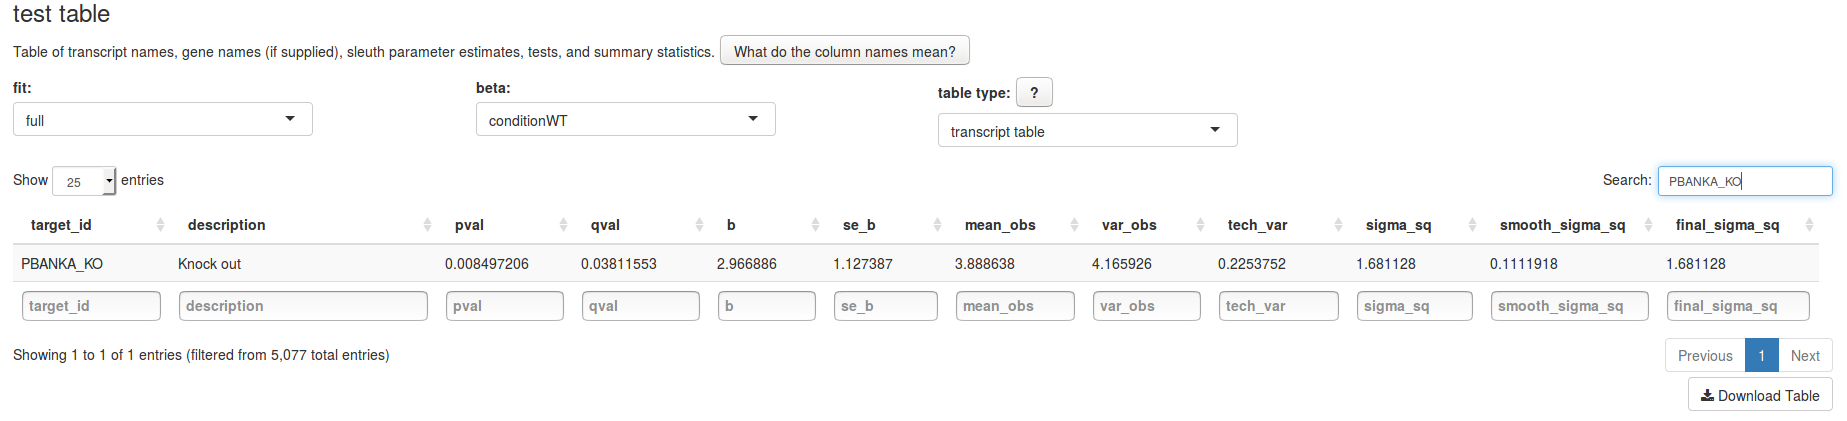
\includegraphics{images/sleuth_test_table.png}
\caption{images/sleuth\_test\_table.png}
\end{figure}

    \textbf{Is there anything unusual about the PBANKA\_KO expression levels
in any of the samples?}

You'll already have seen an indication of this in the genome alignments.
It seems there is partial expression of PBANKA\_KO in KO3.

\newpage

You can look at the expression profiles by going to
\texttt{analyses\ -\textgreater{}\ transcript\ view} and typing
PBANKA\_KO in the search box.

    \begin{figure}[!h]
\centering
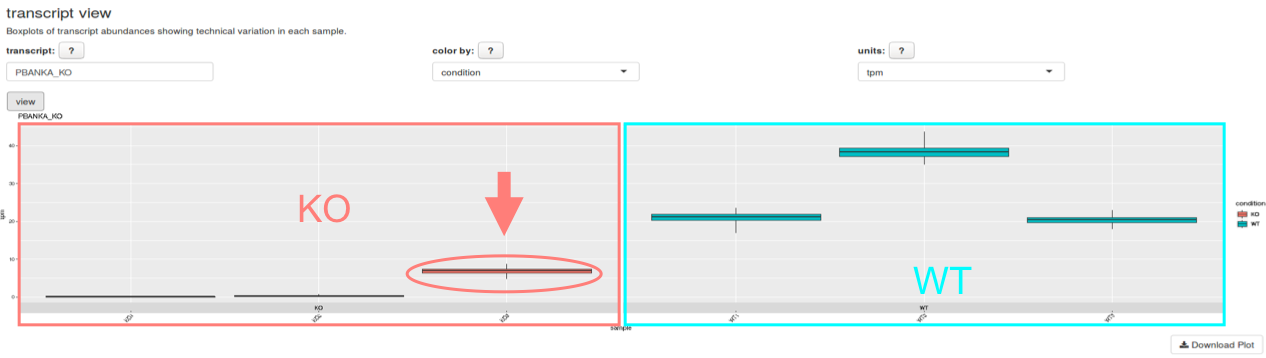
\includegraphics{images/sleuth_transcript_view.png}
\caption{images/sleuth\_transcript\_view.png}
\end{figure}

    \textbf{How many genes are more highly expressed in the WT samples than
in the KO samples?}

\textbf{299}

\begin{terminalinput}
\begin{Verbatim}[commandchars=\\\{\}]
\llap{\color{black}\LARGE\faKeyboardO\hspace{1em}} awk \PYZhy{}F\PY{l+s+s1}{\PYZsq{}\PYZbs{}t\PYZsq{}} \PY{l+s+s1}{\PYZsq{}\PYZdl{}4 \PYZlt{} 0.01 \PYZam{}\PYZam{} \PYZdl{}5 \PYZgt{} 0\PYZsq{}} kallisto.results \PY{p}{|} wc \PYZhy{}l
\end{Verbatim}
\end{terminalinput}


    \textbf{Can you identify which 10 genes are most upregulated in the WT
samples?}

\begin{terminalinput}
\begin{Verbatim}[commandchars=\\\{\}]
\llap{\color{black}\LARGE\faKeyboardO\hspace{1em}} awk \PYZhy{}F\PY{l+s+s1}{\PYZsq{}\PYZbs{}t\PYZsq{}} \PY{l+s+s1}{\PYZsq{}\PYZdl{}4 \PYZlt{} 0.01 \PYZam{}\PYZam{} \PYZdl{}5 \PYZgt{} 0  \PYZob{}OFS=\PYZdq{}\PYZbs{}t\PYZdq{}; print \PYZdl{}1,\PYZdl{}2,\PYZdl{}4,\PYZdl{}5\PYZcb{}\PYZsq{}} \PY{l+s+se}{\PYZbs{}}
        kallisto.results \PY{p}{|} sort \PYZhy{}t\PY{l+s+s1}{\PYZdl{}\PYZsq{}\PYZbs{}t\PYZsq{}} \PYZhy{}k4 \PYZhy{}nr \PY{p}{|} head
\end{Verbatim}
\end{terminalinput}


    \textbf{How many genes are more highly expressed in the KO samples than
in the WT samples?}

\textbf{410}

\begin{terminalinput}
\begin{Verbatim}[commandchars=\\\{\}]
\llap{\color{black}\LARGE\faKeyboardO\hspace{1em}} awk \PYZhy{}F\PY{l+s+s1}{\PYZsq{}\PYZbs{}t\PYZsq{}} \PY{l+s+s1}{\PYZsq{}\PYZdl{}4 \PYZlt{} 0.01 \PYZam{}\PYZam{} \PYZdl{}5 \PYZlt{} 0\PYZsq{}} kallisto.results \PY{p}{|} wc \PYZhy{}l
\end{Verbatim}
\end{terminalinput}


    \textbf{Can you identify which 10 genes are most upregulated in the WT
samples?}

\begin{terminalinput}
\begin{Verbatim}[commandchars=\\\{\}]
\llap{\color{black}\LARGE\faKeyboardO\hspace{1em}} awk \PYZhy{}F\PY{l+s+s1}{\PYZsq{}\PYZbs{}t\PYZsq{}} \PY{l+s+s1}{\PYZsq{}\PYZdl{}4 \PYZlt{} 0.01 \PYZam{}\PYZam{} \PYZdl{}5 \PYZlt{} 0  \PYZob{}OFS=\PYZdq{}\PYZbs{}t\PYZdq{}; print \PYZdl{}1,\PYZdl{}2,\PYZdl{}4,\PYZdl{}5\PYZcb{}\PYZsq{}} \PY{l+s+se}{\PYZbs{}}
        kallisto.results \PY{p}{|} sort \PYZhy{}t\PY{l+s+s1}{\PYZdl{}\PYZsq{}\PYZbs{}t\PYZsq{}} \PYZhy{}k4 \PYZhy{}nr \PY{p}{|} head
\end{Verbatim}
\end{terminalinput}


    \textbf{Write the gene IDs of the significantly differentially expressed
genes to files for the next part of the analysis.}

\begin{terminalinput}
\begin{Verbatim}[commandchars=\\\{\}]
\llap{\color{black}\LARGE\faKeyboardO\hspace{1em}} awk \PYZhy{}F\PY{l+s+s1}{\PYZsq{}\PYZbs{}t\PYZsq{}} \PY{l+s+s1}{\PYZsq{}\PYZdl{}4 \PYZlt{} 0.01 \PYZam{}\PYZam{} \PYZdl{}5 \PYZgt{} 0  \PYZob{}print \PYZdl{}1\PYZcb{}\PYZsq{}} \PY{l+s+se}{\PYZbs{}}
        kallisto.results \PYZgt{} kallisto.WT.sig.genes
\end{Verbatim}
\end{terminalinput}


\begin{terminalinput}
\begin{Verbatim}[commandchars=\\\{\}]
\llap{\color{black}\LARGE\faKeyboardO\hspace{1em}} awk \PYZhy{}F\PY{l+s+s1}{\PYZsq{}\PYZbs{}t\PYZsq{}} \PY{l+s+s1}{\PYZsq{}\PYZdl{}4 \PYZlt{} 0.01 \PYZam{}\PYZam{} \PYZdl{}5 \PYZlt{} 0  \PYZob{}print \PYZdl{}1\PYZcb{}\PYZsq{}} \PY{l+s+se}{\PYZbs{}}
        kallisto.results \PYZgt{} kallisto.KO.sig.genes
\end{Verbatim}
\end{terminalinput}


    \subsection{GO term enrichment
analysis}\label{go-term-enrichment-analysis}

Gene ontology (GO) terms are a dictionary which can be used to assign
functions to a gene or transcript. You can use
\url{http://www.plasmodb.org} to perform a GO term enrichment analysis
(i.e. which terms are significantly more abundant in your differentially
expressed genes than in all of the genes as a whole).

\textbf{Go to \url{http://www.plasmodb.org} in your web browser.}

\textbf{Go to \texttt{My\ Strategies\ -\textgreater{}\ New}.}

\textbf{Go to
\texttt{Annotation,\ curation\ and\ identifiers\ -\textgreater{}\ Gene\ IDs}.}

\textbf{Upload your file of gene IDs that were more highly expressed in
the WT samples.}

\textbf{Go to \texttt{Analyse\ results} (blue button) and
\texttt{GO\ enrichment}.}

\textbf{You want to do a GO analysis using the biological processes (BP).}

\subsubsection{Important questions}\label{important-questions}

\textbf{Which GO terms (biological processes) are enriched in genes with
higher expression in the WT samples?}

You can get this from the table that the analysis generates. You could
say that broadly speaking that this gene is involved in the regulation
of motility, adhesion and the cell cycle.

    \begin{figure}[!h]
\centering
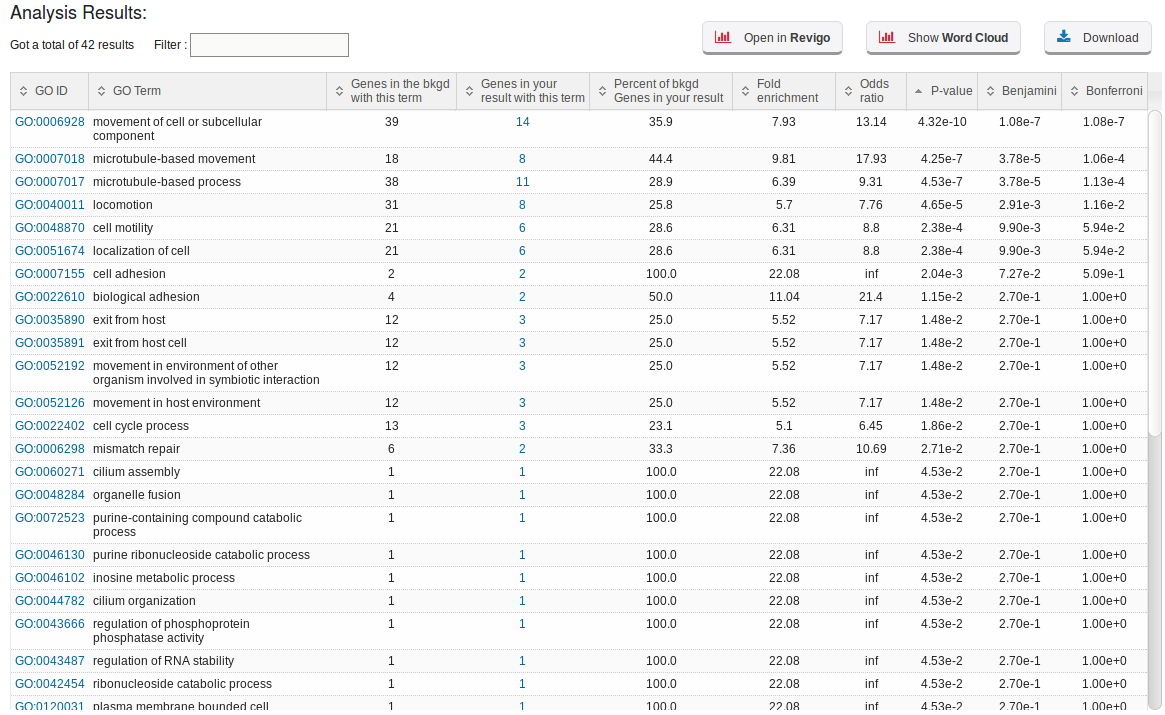
\includegraphics{images/WT_BP_table.png}
\caption{images/WT\_BP\_table.png}
\end{figure}

\newpage

    You can also use some of the other output options to find interesting
ways of displaying this data.

    \begin{figure}[!h]
\centering
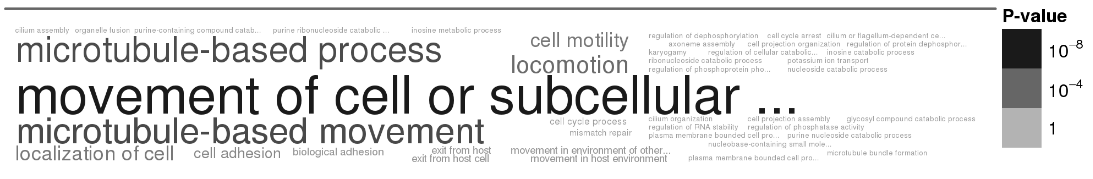
\includegraphics{images/WT_BP_words.png}
\caption{images/WT\_BP\_words.png}
\end{figure}

    \textbf{Which GO terms (biological processes) are enriched in genes with
higher expression in the KO samples?}

    You'll need to run the same analysis with your KO file and look at the
results table. It looks like there are changes in ribosomal processes.

    \begin{figure}[!h]
\centering
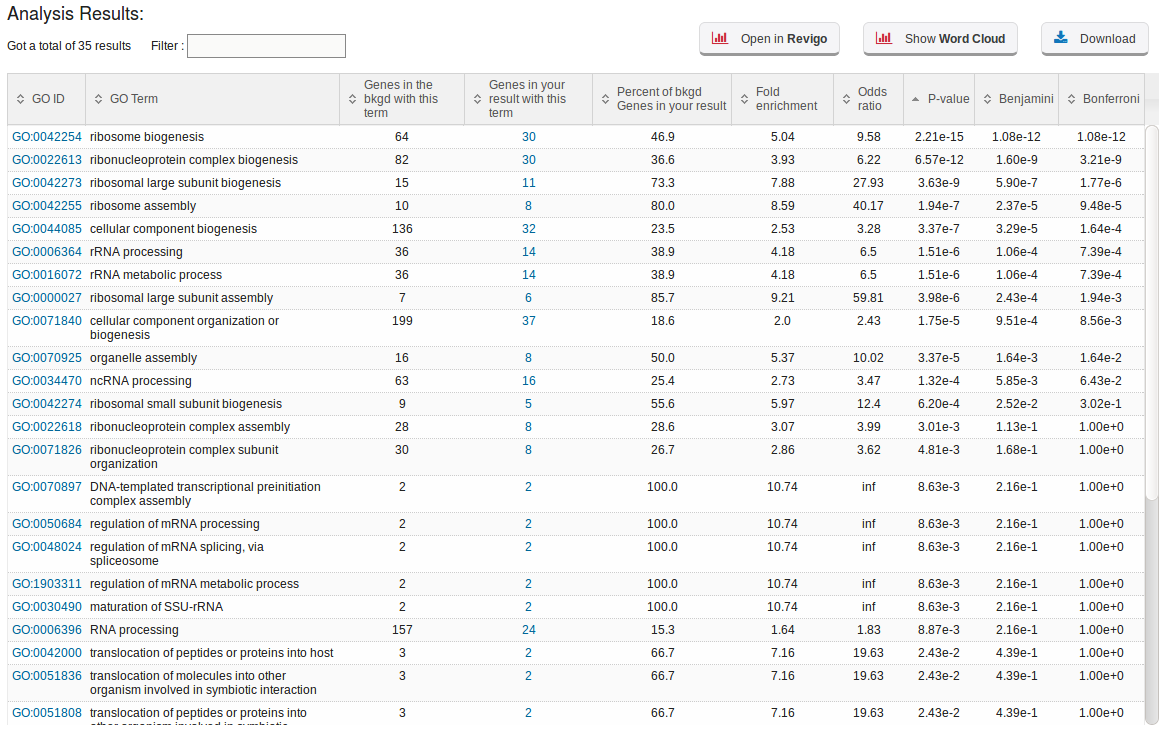
\includegraphics{images/KO_BP_table.png}
\caption{images/KO\_BP\_table.png}
\end{figure}

    And again, there are several useful ways to visualise your results.

    \begin{figure}[!h]
\centering
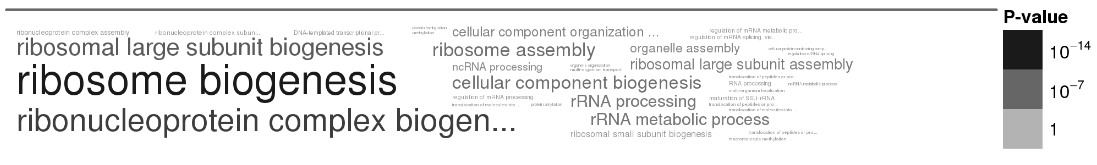
\includegraphics{images/KO_BP_words.png}
\caption{images/KO\_BP\_words.png}
\end{figure}

\newpage

    \subsection{What is PBANKA\_KO?}\label{what-is-pbanka_ko}

So, we've seen the influences of the knock out gene, but what is it?

For this group task, we removed the real name of PBANKA\_KO from all of
the files we gave you. How mean! To get the real name of PBANKA\_KO, we
need the real genome annotation file.

\textbf{Download the real annotation file from the FTP site
(\texttt{Pberghei.gff3.gz}).}

\begin{terminalinput}
\begin{Verbatim}[commandchars=\\\{\}]
\llap{\color{black}\LARGE\faKeyboardO\hspace{1em}} wget ftp://ftp.sanger.ac.uk/pub/project/pathogens/gff3/CURRENT/Pberghei.gff3.gz
\end{Verbatim}
\end{terminalinput}


    Now, earlier on, you will have jotted down the location of PBANKA\_KO in
the genome.

\textbf{Search for a gene with the same co-ordinates as PBANKA\_KO in
the reall annotation file.}

\begin{terminalinput}
\begin{Verbatim}[commandchars=\\\{\}]
\llap{\color{black}\LARGE\faKeyboardO\hspace{1em}} zgrep \PY{l+s+s2}{\PYZdq{}PbANKA\PYZus{}14\PYZus{}v3.*gene.*1416412.*1423431\PYZdq{}} Pberghei.gff3.gz
\end{Verbatim}
\end{terminalinput}


    Looks like PBANKA\_KO is really \textbf{PBANKA\_1437500}, better known
as \textbf{AP2-G}, in disguise!

Looking into the literature, you will find that AP2-G encodes a
transcription factor and plays a role in gametocyte development
(gametogenesis). Thus, it makes sense that knocking out this gene will
result in differential expression of genes involved in cell structure,
cycle and motility.


    % Add a bibliography block to the postdoc



\end{document}
